\subsection*{Question 3}

\noindent First, we mock a \verb|TodoService| object using the \verb|TodoService| interface. Not that the \verb|retrieveTodos()| method of the \verb|TodoService| interface does not have an implementation, all we know is that it must returns a List<String>. We stubb the implementation so that when \verb|todoService.retrieveTodos("Ranga")| is called, a list (allTodos) is returned. Note that the list \verb|allTodos| is a real List<String> object, not a mock. Then we create a real \verb|TodoBusinessImpl| object, giving the mocked \verb|TodoService| object as a parameter. Finally we call \verb|retrieveTodosRelatedToSpring| method of the \verb|TodoBusinessImpl| class on the \verb|todoBusinessImpl| object previously created. For clarity, I joined bellow the implementation of \verb|retrieveTodosRelatedToSpring|. Inside of it is a call to the \verb|retrieveTodos(user)| method. Since the passed parameter is \textit{"Ranga"}, the stubbed method \verb|retrieveTodos| will return the list \verb|allTodos| declared earlier. In that list, two elements have \textit{"Spring"} as a substring. The returned element \textit{filteredTodos} will hence be a list containing two elements. Asserting that the size of that list is equal to 2 will then be true. 
\begin{center}
        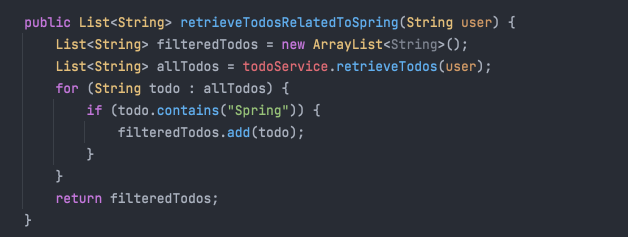
\includegraphics[width=0.9\textwidth]{img/partc.png}
        \noindent  Implementation of the \verb|retrieveTodosRelatedToSpring| method
\end{center}